\documentclass{article}
\usepackage{v-test-paper}
\usepackage{mathtools}

\title{\textsc{Coordinate System}}

\begin{document}
\maketitle

\begin{itemize}
    \item Location of a point on a line
    \begin{quote}
        \textit{
            Imagine a world where you can only move in two directions: forward and backward. You can't move left or right, up or down—only along a single straight path. This path is called the x-axis. The x-axis is a horizontal line that extends infinitely in both directions. \\[2mm]
            In this one-dimensional world, we can describe the location of any point using a single number, which we call the coordinate of that point. This number tells us exactly how far along the x-axis the point is from a specific reference point known as the origin. The origin is the center point of the x-axis and has a coordinate of $0$.\\[2mm]
            If a point has a positive coordinate, it means the point is to the right of the origin. If a point has a negative coordinate, it means the point is to the left of the origin. The greater the number, the further the point is from the origin.
        }
    \end{quote}

        \begin{center}
            \begin{tikzpicture}
                \tzaxes(-5, 0)(5, 0.15){$x$}{}
                \tzticks{-4/$-4$, -3/$-3$, -2/$-2$, -1/$-1$, 0/$0$, 1/$1$, 2/$2$, 3/$3$, 4/$4$}{}
                \tzticks*{-4, -3, -2, -1, 1, 2, 3, 4}{}
            \end{tikzpicture}
            \begin{tikzpicture}
                \tzaxes(-5, 0)(5, 0.15){$x$}{}
                \tzticks{-2.5/$x_1$, 2.5/$x_2$}{}
                \tzticks*{-2.5, 0, 2.5}{}
                \tzline[|<->|]<0, -0.75>(-2.5, 0)(2.5, 0){$x_2 - x_1$}[mb]
            \end{tikzpicture}
        \end{center}

    \item Location of a point in a plane
    \begin{quote}
        \textit{
            Now, imagine a world where you can move not just forward and backward, but also left and right. This world is two-dimensional, meaning it has two directions or axes along which you can move: the x-axis and the y-axis.\\[2mm]
            The x-axis is a horizontal line that runs from left to right, and the y-axis is a vertical line that runs from bottom to top. These two lines intersect at a point called the origin, which has the coordinates (0, 0).
            In this two-dimensional world, we can describe the location of any point using a pair of numbers called coordinates. These coordinates are written as (x, y):\\[2mm]
            The first number, x, tells us how far along the x-axis the point is from the origin. A positive x value means the point is to the right of the origin, while a negative x value means the point is to the left.
            The second number, y, tells us how far along the y-axis the point is from the origin. A positive y value means the point is above the origin, while a negative y value means the point is below.
        }
    \end{quote}

        \begin{center}
            \begin{tikzpicture}
                \tzaxes(-5, -3)(5, 4){$x$}{$y$}
                \tzticks*{-4, -3, -2, -1, 1, 2, 3, 4}{-2, -1, 1, 2, 3}
                \tzcoor*(0, 0)(O){$O$}[bl]
                \tzcoor*(2, 3)(P){$P(2,3)$}[ar]
                \tzline[|<->|]<0, -0.5>(0, 0)(2, 0){$2$}[mb]
                \tzline[|<->|]<2.5, 0>(0, 0)(0, 3){$3$}[mr]
            \end{tikzpicture}
        \end{center}

        \textbf{Coordinates of a point $P(x, y)$:} \\
        
        \begin{itemize}
            \item \textbf{Distance between two points:}
                \begin{center}
                    \begin{tikzpicture}
                        \tzaxes(-2, -1.5)(7, 4){$x$}{$y$}
                        \tzcoor*(0, 0)(O){$O$}[bl]
                        \tzcoor*(2, 3)(P){$P(x_1, y_1)$}[ar]
                        \tzcoor*(5, 1)(Q){$Q(x_2, y_2)$}[ar]
                        \tzline[dashed](2, 1)(5, 1){$x_2-x_1$}[mb]
                        \tzline[dashed](2, 1)(2, 3){$y_1-y_2$}[ml]
                        \tzline(P)(Q){$d$}[ma]
                        \tzline[|<->|]<0, -0.5>(0, 0)(2, 0){$x_1$}[mb]
                        \tzline[|<->|]<0, -1>(0, 0)(5, 0){$x_2$}[mb]
                        \tzline[|<->|]<-0.5, 0>(0, 0)(0, 1){$y_2$}[ml]
                        \tzline[|<->|]<-1, 0>(0, 0)(0, 3){$y_1$}[ml]
                    \end{tikzpicture}
                \end{center}
                \begin{align*}
                    \intertext{Distance between two points $P(x_1, y_1)$ and $Q(x_2, y_2)$:}
                    \intertext{Using Pythagoras theorem:}
                    \Aboxed{d &= \sqrt{(x_2 - x_1)^2 + (y_2 - y_1)^2}}
                \end{align*}

            \item \textbf{Midpoint of a line segment:}
                \begin{center}
                    \begin{tikzpicture}
                        \tzcoor*(2, 3)(P){$P(x_1, y_1)$}[ar]
                        \tzcoor*(5, 1)(Q){$Q(x_2, y_2)$}[ar]
                        \tzcoor*(3.5, 2)(M){$M(x_m, y_m)$}[ar]
                        \tzline[dashed](2, 1)(5, 1){$x_2-x_1$}[mb]
                        \tzline[dashed](2, 1)(2, 3){$y_1-y_2$}[ml]
                        \tzline(P)(Q)
                        \tzline[dashed](2, 2)(M){$x_m-x_1$}[mb]
                        \tzline[dashed, |<->|]<-1.5, 0>(2, 2)(2, 3){$y_1-y_m$}[ml]
                    \end{tikzpicture}
                \end{center}
                \begin{align*}
                    \intertext{Midpoint of a line segment $P(x_1, y_1)$ and $Q(x_2, y_2)$:}
                    \intertext{From the above diagram, we can see that both the triangles are similar.}
                    \intertext{Therefore,}
                    \frac{y_1-y_m}{y_1-y_2} &= \frac{x_m-x_1}{x_2-x_1} = \frac{PM}{PQ} \\
                    \intertext{As the midpoint divides the line segment into two equal parts,}
                    \frac{y_1-y_m}{y_1-y_2} &= \frac{x_m-x_1}{x_2-x_1} = \frac{1}{2}
                \end{align*}
                \begin{align*}
                    \intertext{Solve for $x_m$ and $y_m$:}
                    \frac{x_m - x_1}{x_2 - x_1} &= \frac{1}{2}  &\text{and}&& \frac{y_1 - y_m}{y_1 - y_2} &= \frac{1}{2} \\
                    x_m - x_1 &= \frac{x_2 - x_1}{2}  &\text{and}&& y_1 - y_m &= \frac{y_1 - y_2}{2} \\
                    x_m &= \frac{x_1 + x_2}{2}  &\text{and}&&  y_m &= \frac{y_1 + y_2}{2}
                \end{align*}
                \begin{align*}
                    \Aboxed{M(x_m, y_m) &= \left(\frac{x_1 + x_2}{2}, \frac{y_1 + y_2}{2}\right)}
                \end{align*}
        \end{itemize}

\end{itemize}
\pagebreak

\begin{center}
    \textsc{\Large\textbf{Slope of a line}}
\end{center}
    \begin{center}
        \begin{tikzpicture}
            \tzaxes(-2, -1.5)(7, 4){$x$}{$y$}
            \tzline"L1"(0, 0)(6, 4){$L_1(x)$}[ar]
            \tzline"L2"(0, 0)(6, 2){$L_2(x)$}[ar]
            \tzline[dashed]"DL"(4, 0)(4, 4)
            \tzXpoint{DL}{L1}(X1)
            \tzXpoint{DL}{L2}(X2)
            \tzdot*(X1)
            \tzdot*(X2)
            \tzline[|<->|]<0, -0.5>(0, 0)(4, 0){$\Delta x$}[mb]
            \tzline[|<->|]<0.5, 0>(4, 0)(X2){$\Delta y_2$}[mr]
            \tzline[|<->|]<1.5, 0>(4, 0)(X1){$\Delta y_1$}[mr]
        \end{tikzpicture}
    \end{center}
    \begin{quote}
        \textit{
            The slope of a line is a measure of its steepness and direction, and it can be interpreted as the rate of change of the line. It is calculated as the ratio of the vertical change to the horizontal change between two distinct points on the line.\\[2mm]
            In the above diagram $L_1$ and $L_2$ are two lines, $\Delta x$ is the horizontal change, and $\Delta y_1$ and $\Delta y_2$ are the vertical changes of the lines $L_1$ and $L_2$ respectively.\\[2mm]
            As you can see $\Delta y_1 > \Delta y_2$ and $\Delta x$ is the same for both the lines. Therefore, the slope of the line $L_1$ is greater than the slope of the line $L_2$.\\[2mm]
            Here, for both the lines $L_1$ and $L_2$, for $\Delta x > 0$, $\Delta y_1 \textit{ and } \Delta y_2$ are positive. Therefore, the slope of the line is positive.
        }
    \end{quote}
    \begin{itemize}
        \item But slope can be negative if $\Delta y < 0$ for $\Delta x > 0$.
            \begin{center}
                \begin{tikzpicture}
                    \tzaxes(-2, -1)(7, 4){$x$}{$y$}
                    \tzcoors*(1,1)(A)(1,2)(B)(3,1)(C);
                    \tzLFn(B)(C)[-1:5]
                    \tzline[dashed](A)(B)
                    \tzline[dashed](A)(C)
                    \tzline[|<->|]<-0.25, 0>(A)(B){$\Delta y$}[ml]
                    \tzline[|<->|]<0, -0.25>(A)(C){$\Delta x$}[mb]
                \end{tikzpicture}
            \end{center}

        \item Slope can be zero if $\Delta y = 0$ for all $\Delta x \neq 0$.
            \begin{center}
                \begin{tikzpicture}
                    \tzaxes(-2, -1)(7, 3.5){$x$}{$y$}
                    \tzcoors*(1, 2)(A)(3, 2)(B);
                    \tzLFn(A)(B)[-1:5]
                    \tzline[|<->|]<0, -0.25>(A)(B){$\Delta x$}[mb]
                \end{tikzpicture}
            \end{center}

        \item Slope can be undefined if $\Delta x = 0$\\
            In this case, the line is vertical, meaning the slope tends to infinity. This situation violates the definition of slope because the slope is the ratio of the vertical change to the horizontal change. However, when the horizontal change is zero but the vertical change is not zero, this ratio becomes undefined.
            \begin{center}
                \begin{tikzpicture}
                    \tzaxes(-2, -1)(7, 4){$x$}{$y$}
                    \tzcoors*(1, 1)(A)(1, 3)(B);
                    % \tzLFn(A)(B)[-1:5]
                    \tzline($(A)+(0, -1.5)$)($(B)+(0, 1)$)
                    \tzline[|<->|]<-0.25, 0>(A)(B){$\Delta y$}[ml]
                \end{tikzpicture}
            \end{center}
    \end{itemize}
    % \pagebreak
\vspace*{10mm}
    \begin{center}
        \textsc{Slope of a line passing through two points $P(x_1, y_1)$ and $Q(x_2, y_2)$}\\[10mm]
        \begin{tikzpicture}
            \tzaxes(-2, -1)(7, 4){$x$}{$y$}
            \tzcoors*(4,1)(A)(1,1)(B){$P(x_1, y_1)$}[al](4,3)(C){$Q(x_2, y_2)$}[al];
            \tzLFn(B)(C)[-1:5]
            \tzline[dashed](A)(B)
            \tzline[dashed](A)(C)
            \tzline[|<->|]<0, -0.5>(A)(B){$\Delta x$}[mb]
            \tzline[|<->|]<0.5, 0>(A)(C){$\Delta y$}[mr]
            \tzanglemark(A)(B)(C){$\theta$}(15pt)
        \end{tikzpicture}
    \end{center}
    \begin{align*}
        \intertext{Slope of a line passing through two points $P(x_1, y_1)$ and $Q(x_2, y_2)$:}
        \textit{Slope(m) } &= \frac{\Delta y}{\Delta x} \\
        \intertext{From the above diagram,}
        \tan \theta &= \frac{\Delta y}{\Delta x} \\
        \intertext{Therefore,}
        \Aboxed{m &= \tan \theta = \frac{y_2 - y_1}{x_2 - x_1}}
        \intertext{Be careful, $\theta$ is the angle between the line and the positive x-axis in anti-clockwise direction.}
    \end{align*}


\end{document}